% Part 2 chapter (replaces the Koide section of p2_15_particle_masses.tex). Carries "Three Charged Lepton Generations and the Koide Ratio
% from Horizon Information Equipartition on a Charge Orbit" (22 Apr 2026; docs/papers/Koide_Mahaffey.pdf, PDF text 839 lines, read in full
% 2026-10-02) and, for equation forms and figures only, its earlier conditional version (Koide_Paper.tex = Koide_Paper_revised.tex, 359 lines;
% Koide_ratio_from_holographic_boundary.pdf, 366 lines; generate_koide_figures.py, 101 lines). Corrections: PAPER_ERRATA KO1-KO4 and KO5-KO8
% (MANIFEST_particle.md). Numbers: docs/verification/scripts/verify_particle_book.py (K1-K18) and verify_koide.py. Figures:
% docs/book/figscripts/fig_p2_particle.py.
\chapter{Three charged leptons and the Koide relation}\label{ch:koide}

\section*{The place}
The Standard Model takes the three charged-lepton masses as inputs. One empirical relation among them has held for four decades without a
derivation: Koide's relation. This chapter states the relation and its geometry, then follows one route that would explain it. The route
starts from IAM's Law (Chapter~\ref{ch:iams_law}): a classical record is written to the nearest surface and costs $\kB T\ln2$ per bit. It
ends with the value $2/3$ and a bound on the number of generations. Every step carries its status. The algebra is exact. The physical steps
that feed it are assumptions or conjectures, and one of them, the phase offset, is an open problem that the route does not close.

\section{Koide's relation}\label{sec:ko:relation}
For the charged-lepton pole masses define~\cite{Koide1982,Koide1983,Koide1983b}
\begin{equation}
Q\equiv\frac{m_e+m_\mu+m_\tau}{\big(\sqrt{m_e}+\sqrt{m_\mu}+\sqrt{m_\tau}\big)^2}.\label{eq:ko:Q}
\end{equation}
For any three positive masses $1/3\le Q<1$: $Q=1/3$ when the masses are equal and $Q\to1$ when one mass dominates. \derived{} The measured
masses sit almost exactly in the middle of that range, at $2/3$ (Table~\ref{tab:ko:masses}).

\begin{table}[htbp]\centering\small
\caption{Charged-lepton pole masses and the Koide ratio. Masses from the Particle Data Group~\cite{PDG2024}; the 2022 value of $m_\tau$~\cite{PDG2022}
is shown for comparison. Recomputed in \texttt{verify\_particle\_book.py} (K1, K4, K8).}\label{tab:ko:masses}
\begin{tabular}{lll}\toprule
quantity & value & label\\\midrule
$m_e$ & $0.51099895000(15)$\,MeV & \observed\\
$m_\mu$ & $105.6583755(23)$\,MeV & \observed\\
$m_\tau$ (2024) & $1776.93\pm0.09$\,MeV & \observed\\
$m_\tau$ (2022) & $1776.86\pm0.12$\,MeV & \observed\\\midrule
$Q$ with the 2024 masses & $0.66666446\pm0.00000508$ & \calc\\
$2/3-Q$ & $2.2\times10^{-6}$, that is $0.43\sigma$ & \calc\\
$Q$ with the 2022 $m_\tau$ & $0.66666051$ ($2/3-Q=6.2\times10^{-6}$) & \calc\\\bottomrule
\end{tabular}
\end{table}

The uncertainty on $Q$ comes almost entirely from $m_\tau$. With the 2024 average the relation holds to $2.2\times10^{-6}$, inside one standard
deviation. \observed{} No symmetry of the Standard Model requires it. \observed

\paragraph{Pole masses and running.} The relation is stated for pole masses. Running masses at a common scale do not satisfy it at this
level~\cite{Xing2006}. The size of the effect follows from one-loop QED alone. In the $\overline{\rm MS}$ scheme
$\bar m(\mu)=M\,[1-(\alpha/\pi)(1+\tfrac32\ln(\mu/M))]$, and the logarithm differs from lepton to lepton. With $\alpha$ held at $1/137.036$,
\begin{equation}
Q(\mu=m_\tau)=0.667824,\qquad Q(\mu=M_Z)=0.667840,
\end{equation}
a departure of $1.2\times10^{-3}$ from $2/3$, some 500 times the present uncertainty. \calc{} The agreement at $10^{-6}$ is therefore a property of
the pole masses. Why the pole masses, and not the masses at some other scale, is open; one published mechanism cancels the QED correction with a
family gauge symmetry~\cite{Sumino2009}. \openprob

\section{The square-root vector and its angle}\label{sec:ko:angle}
Write the square roots as a vector in a three-dimensional flavour space,
\begin{equation}
\vec s=\big(\sqrt{m_e},\sqrt{m_\mu},\sqrt{m_\tau}\big)=(0.7148,\;10.2790,\;42.1536)\ {\rm MeV}^{1/2}.
\end{equation}
\calc{} Let $\theta$ be its angle to the democratic direction $(1,1,1)$. Then
\begin{equation}
\cos^2\theta=\frac{(\vec s\cdot(1,1,1))^2}{3\,|\vec s|^2}=\frac{(\sum_k\sqrt{m_k})^2}{3\sum_km_k}=\frac{1}{3Q}.\label{eq:ko:angle}
\end{equation}
\derived{} So $Q=2/3$ is the statement $\cos^2\theta=1/2$: the square-root vector lies at exactly $45^\circ$ to $(1,1,1)$~\cite{Foot1994}. The measured
vector lies at $44.99991^\circ$. \calc{} Figure~\ref{fig:ko:flavour} shows the vector, the diagonal, and the circle of all vectors of the same
length along the diagonal that lie at $45^\circ$.

\begin{figure}[htbp]\centering
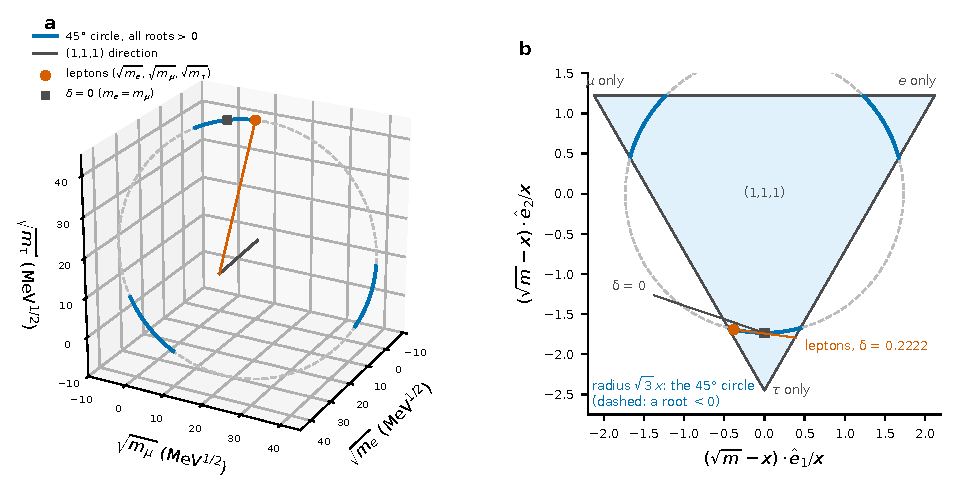
\includegraphics[width=\textwidth]{figures/part2/fig_koide_flavour.pdf}
\caption[The charged leptons in flavour space]{(a) The square-root mass vector $(\sqrt{m_e},\sqrt{m_\mu},\sqrt{m_\tau})=(0.7148,10.2790,42.1536)$\,MeV$^{1/2}$
(PDG 2024~\cite{PDG2024}; orange point and line from the origin), the $(1,1,1)$ direction (grey), and the circle of vectors at $45^\circ$ to it with
the same projection $3x$ on the diagonal, $x^2=313.85$\,MeV (blue where all three components are positive, dashed where one is negative). The
square marks the offset $\delta=0$, where $m_e=m_\mu$. (b) The same circle in the plane $\sum_k\sqrt{m_k}=3x$, in units of $x$: the shaded triangle is
the region of positive roots, with one lepton alone at each vertex; the circle has radius $\sqrt3\,x$ and leaves the triangle on three arcs. The
measured leptons lie near the $\tau$ vertex, close to the edge where $\sqrt{m_e}=0$. \calc}\label{fig:ko:flavour}
\end{figure}

\section{The circle and the three phases}\label{sec:ko:circle}
Any three positive square roots can be written as samples of one function on a circle at three equally spaced phases~\cite{Brannen2006}:
\begin{equation}
\sqrt{m_k}=x\big[1+r\cos(\delta+2\pi k/3)\big],\qquad k=0,1,2.\label{eq:ko:param}
\end{equation}
The three parameters $(x,r,\delta)$ carry the same information as the three masses; the form is a change of variables, not a model.
\derived{} The phases $\phi_k=\delta+2\pi k/3$ are the orbit of the cyclic group $Z_3$. For $Z_3$ phases, at every $\delta$,
\begin{equation}
\sum_k\cos\phi_k=0,\qquad\sum_k\cos^2\phi_k=\tfrac32,\label{eq:ko:Z3}
\end{equation}
so $\sum_k\sqrt{m_k}=3x$, $\sum_km_k=3x^2(1+r^2/2)$, and
\begin{equation}
Q=\frac13\Big(1+\frac{r^2}{2}\Big).\label{eq:ko:Qr}
\end{equation}
\derived{} Koide's relation is therefore the single statement $r=\sqrt2$. It fixes neither the scale $x$ nor the offset $\delta$.

The measured masses give (Table~\ref{tab:ko:fit}) $x=17.71584$\,MeV$^{1/2}$, $x^2=313.851$\,MeV, $r=1.414209$ against $\sqrt2=1.414214$, and
$\delta=0.222225$\,rad, with the $\tau$ at $k=0$, the electron at $k=1$ and the muon at $k=2$. \calc{} The offset is close to $2/9=0.222222$, a
coincidence noted in the literature~\cite{Brannen2006}: the difference is $2.5\times10^{-6}$\,rad, $0.41$ standard deviations of the offset as $m_\tau$
fixes it. \calc{} The coincidence has no explanation. \openprob

\section{The encoding on a charge orbit}\label{sec:ko:encoding}
The route to $r=\sqrt2$ takes Eq.~\eqref{eq:ko:param} literally. The circle is a physical orbit, the three leptons are three phase states on it, and
the amplitude ratio is set by how information is shared between the two parts of the encoding. The chain has seven steps. Each is given in full
with its status.

\subsection{Step 1: the charge orbit}
In the gauge/gravity correspondence a bulk gauge field of charge $Q$ corresponds to a global $U(1)$ symmetry of the boundary theory with the same
charge~\cite{Maldacena1999}. For a fixed nonzero charge sector, $|Q|=1$, the boundary degrees of freedom relevant to that sector are taken to lie on
a one-parameter orbit $S^1$ inside the two-sphere of the boundary, parametrised by one phase $\phi$. All states of the same $|Q|$ share the orbit.
This reduction rests on firm ground in anti-de Sitter space. Its de Sitter counterpart is not established. \conjecture{} Only the structural fact
is used: a fixed nonzero charge restricts to a circle carrying one phase variable.

\subsection{Step 2: records are written to the boundary}
Decoherence turns $|\psi\rangle_S|E_0\rangle$ into $\sum_ic_i|s_i\rangle|E_i\rangle$; once the environmental records $|E_i\rangle$ are orthogonal the
reduced state of $S$ is diagonal in the pointer basis~\cite{Zurek2003}. Restoring the coherences would require erasing the records, which costs at
least $\kB T\ln2$ per bit~\cite{Landauer1961}. The transition is irreversible and each event produces $\log_2N$ bits for $N$ distinguishable
outcomes. \derived{} (standard). The record must be kept where an outside observer can reach it. The causal boundary of a region is a
two-dimensional surface; the interior is not accessible from outside. Taking the record to the boundary gives $S\propto A$. This is the holographic
argument~\cite{tHooft1993,Susskind1995}. For a black hole the area law is established~\cite{Bekenstein1973,Hawking1975}; for an arbitrary region
containing a decoherence event it is a conjecture. \conjecture

\subsection{Step 3: the coefficient $1/4$}
Near a horizon the Rindler metric is $ds^2=-\kappa^2\rho^2dt^2+d\rho^2+dx_\perp^2$. In Euclidean time $t\to-i\tau$ the $(\rho,\kappa\tau)$ plane is a
cone, regular at $\rho=0$ only if $\kappa\tau$ has period $2\pi$. The thermal period then fixes the temperature~\cite{Unruh1976,BisognanoWichmann1976},
\begin{equation}
T=\frac{\hbar\kappa}{2\pi\kB}.\label{eq:ko:TU}
\end{equation}
The Einstein equations carry $8\pi G/c^4$: $4\pi$ from the solid angle in Poisson's equation and a factor 2 from the trace term. Jacobson's derivation
of the Einstein equations from $\delta Q=T\,dS$ on local Rindler horizons~\cite{Jacobson1995}, with $S=\eta A$, gives
\begin{equation}
\frac{\hbar\eta}{2\pi}=\frac{c^3}{8\pi G}\quad\Longrightarrow\quad\eta=\frac{c^3}{4\hbar G}=\frac1{4\lP^2}.\label{eq:ko:eta}
\end{equation}
\derived{} The $1/4$ is the ratio $2\pi/8\pi$ of the Euclidean period to the Einstein normalisation.

\subsection{Step 4: one unit per minimum area}
Absorbing the energy $\kB T$ at a horizon of temperature $T$ raises its entropy by $\delta S=1$ (in units of $\kB$) by the first law, and so its
area by $\delta A_{\min}=1/\eta=4\lP^2$:
\begin{equation}
\eta\,\delta A_{\min}=1.\label{eq:ko:onebit}
\end{equation}
\derived{} The result holds at every horizon and needs no choice of surface gravity. It restates the area law; it adds no new input. The unit is
the nat. One bit, priced at $\kB T\ln2$, corresponds to $4\lP^2\ln2$. \derived

\subsection{Step 5: equal weights from maximum entropy}
Let the boundary support $K$ independent encoding channels with information weights $w_k\ge0$ and fixed total $W=\sum_kw_k$, set by the area
through Eq.~\eqref{eq:ko:onebit}. Treat $p_k=w_k/W$ as a distribution and maximise its Shannon entropy $H=-\sum_kp_k\log_2p_k$ under
$\sum_kp_k=1$:
\begin{equation}
\frac{\partial}{\partial p_k}\Big(H-\lambda\sum_jp_j\Big)=0\quad\Longrightarrow\quad p_k=\frac1K,\qquad w_k=\frac WK.\label{eq:ko:maxent}
\end{equation}
\derived{} (given the set-up). For two channels, $w_a=w_b=W/2$. Two identifications make this physics rather than arithmetic: that the
weights of the encoding channels form a distribution to which the maximum-entropy principle applies, and that this is the same principle that
makes the Bekenstein--Hawking entropy the bound at fixed area. Neither is established. \conjecture

\subsection{Step 6: two channels on the orbit}
The most general encoding of the square root on $S^1$ is a Fourier series,
\begin{equation}
\sqrt{m(\phi)}=a_0+\sum_{n\ge1}\big(a_n\cos n\phi+b_n\sin n\phi\big).\label{eq:ko:fourier}
\end{equation}
Mode $n$ carries the orbit-averaged gradient density $\langle|\partial_\phi\cos n\phi|^2\rangle=n^2/2$, so its gradient cost at unit amplitude is
\begin{equation}
E^{\rm grad}_n=\frac{n^2}{2}\,\omega_0^2,\label{eq:ko:grad}
\end{equation}
with $\omega_0$ the gradient unit set by the orbit circumference; the constant mode costs nothing. \derived{} At zero encoding temperature only the
constant mode and the first harmonic are populated. At a finite encoding temperature the higher modes are suppressed as
\begin{equation}
\frac{w_n}{w_1}\sim\exp\!\Big[-\frac{(n^2-1)\,\omega_0^2}{2\kB T_{\rm enc}}\Big].\label{eq:ko:boltz}
\end{equation}
\conjecture{} (the encoding temperature and $\omega_0$ are not specified). A reflection symmetry $\phi\to-\phi$ removes $\sin\phi$, and the phase
origin is placed at the maximum of $\sqrt{m(\phi)}$. The ground-state encoding is then
\begin{equation}
\sqrt{m(\phi)}=x+y\cos\phi,\qquad x>0.\label{eq:ko:two}
\end{equation}
\conjecture{} The two modes are orthogonal on the orbit, $\langle\cos\phi\rangle=0$, so they are independent channels in the sense of Step~5.
\derived

Two consequences of sampling at three points matter here. First, on $Z_3$ the second harmonic is indistinguishable from the first:
$\cos(2\phi_k)=\cos(2\pi k/3-2\delta)$ at every $k$. A $\cos2\phi$ admixture of amplitude $a_2$ changes the effective first harmonic of the three
samples and shifts $Q$ by up to $0.67\,a_2/y$ (K15). \calc{} The measured $Q$ therefore bounds $a_2/y\lesssim10^{-5}$, a weight ratio
$w_2/w_1\lesssim10^{-10}$, which by Eq.~\eqref{eq:ko:boltz} needs $\kB T_{\rm enc}\lesssim\omega_0^2/15$. \calc{} Second, three masses cannot
reveal which harmonics the continuous encoding contains: any three samples fit Eq.~\eqref{eq:ko:param} exactly. The truncation to two modes is a
statement about the orbit, not one the masses can test. \derived

\subsection{Step 7: the amplitude ratio}
The information weight of each channel is identified with its squared amplitude averaged over the orbit (Parseval on $S^1$):
\begin{equation}
w_{\rm DC}=\frac1{2\pi}\int_0^{2\pi}x^2\,d\phi=x^2,\qquad w_{\rm harm}=\frac1{2\pi}\int_0^{2\pi}(y\cos\phi)^2\,d\phi=\frac{y^2}{2}.\label{eq:ko:weights}
\end{equation}
The identification of information weight with mean squared amplitude is what carries the horizon equipartition onto the orbit.
\conjecture{} Equal weights, Eq.~\eqref{eq:ko:maxent} with $K=2$, then give
\begin{equation}
x^2=\frac{y^2}{2}\quad\Longrightarrow\quad\frac yx=\sqrt2.\label{eq:ko:ratio}
\end{equation}
\derived{} (given Steps 1--7). No parameter is adjusted to the masses. The same ratio follows from a different identification: the constant
part and the modulation as the two halves of the virial partition of a $1/r$ potential, $2x^2=y^2$ (Chapter~\ref{ch:virial}). That route is an
analogy, not a derivation. \analogy

\section{The number of generations}\label{sec:ko:count}
Place $n$ generations at equally spaced phases on the orbit, $\phi_k=\delta+2\pi k/n$, with $m_k=(x+y\cos\phi_k)^2$. The condition imposed on the
encoding is that every amplitude is positive,
\begin{equation}
\sqrt{m_k}=x\big(1+\sqrt2\cos\phi_k\big)>0\quad\Longleftrightarrow\quad|\phi_k-\pi|>\pi/4\ ({\rm mod}\ 2\pi).\label{eq:ko:pos}
\end{equation}
Each phase must avoid an arc of width $\pi/2$ centred on $\pi$.

\paragraph{Theorem 1 (generation count).} With $y/x=\sqrt2$:
\begin{enumerate}
\item No $n\ge4$ is admissible for any offset $\delta$.
\item $n=2$ is admissible when $|\cos\delta|<1/\sqrt2$, that is for half of all offsets.
\item $n=3$ is admissible when $\delta$ lies within $\pi/12$ of a multiple of $2\pi/3$, a quarter of all offsets.
\item At $\delta=0$, $n=3$ is the only admissible count. At the measured offset $\delta=0.2222$ it is also the only one.
\end{enumerate}
\emph{Proof.} Any closed arc of length $2\pi/n$ contains at least one of $n$ equally spaced points. The closed arc
$|\phi-\pi|\le\pi/4$ has length $\pi/2\ge2\pi/n$ for $n\ge4$, so for every $\delta$ some phase has $1+\sqrt2\cos\phi_k\le0$. For $n=2$ the phases are $\delta$ and $\delta+\pi$; both amplitudes are positive when $1\pm\sqrt2\cos\delta>0$, that is
$|\cos\delta|<1/\sqrt2$. For $n=3$ the three points spaced by $2\pi/3$ miss an arc of width $\pi/2$ only when none lies within $\pi/4$ of $\pi$,
which leaves windows of total width $3\times(2\pi/3-\pi/2)=\pi/2$, centred where one phase sits at the maximum. The fraction of offsets that
admit $n$ phases is $\max(0,1-n/4)$: 0.50, 0.25 and 0 for $n=2$, 3 and $\ge4$ (K10). At $\delta=0$, $n=2$ fails because the phase $\pi$ is
present, $1-\sqrt2<0$; at $\delta=0.2222$, $\cos\delta=0.975>1/\sqrt2$ and $n=2$ fails again (K18). For $n=3$ at $\delta=0$ the amplitudes are
$x(1+\sqrt2)$ and twice $x(1-\sqrt2/2)$, all positive. $\square$ \derived

So the encoding allows at most three generations at any offset. At $\delta=0$, the offset of Step~6, and at the measured
offset, it allows exactly three. Two points limit the reach of the theorem. The masses themselves are squares and are positive whatever the
sign of the amplitude; the theorem constrains the sign of the encoded amplitude, which is an assumption about the encoding. \derived{} With signed
amplitudes allowed, equal weights give $Q_n=2/n$ for every $n\ge3$ (K11), so the value $2/3$ belongs to three generations, but the count is no
longer bounded. \calc

\section{The Koide value}\label{sec:ko:value}
\paragraph{Theorem 2 (Koide ratio).} For $n=3$ phases $\phi_k=\delta+2\pi k/3$ and $m_k=(x+y\cos\phi_k)^2$ with $y^2/x^2=2$, $Q=2/3$ exactly, for
every $\delta$ at which all amplitudes are positive.

\emph{Proof.} By Eq.~\eqref{eq:ko:Z3}, $\sum_k\sqrt{m_k}=\sum_k(x+y\cos\phi_k)=3x$ and
$\sum_km_k=3x^2+y^2\sum_k\cos^2\phi_k=3x^2+\tfrac32y^2$. Hence
\begin{equation}
Q=\frac{3x^2+\tfrac32y^2}{(3x)^2}=\frac13\Big(1+\frac{y^2}{2x^2}\Big)=\frac13(1+1)=\frac23.\label{eq:ko:thm2}
\end{equation}
$\square$ \derived

The two theorems form the algebraic layer. Given the two-channel form and $y/x=\sqrt2$, they are exact, and a reader can check them without the
holographic steps. The model layer is Steps 1--7: the charge orbit, the boundary record, the area law, equipartition by maximum entropy, the
two-mode ground state and the Parseval identification. Every step of that layer is an assumption or a conjecture.

\section{The offset}\label{sec:ko:offset}
Step~6 fixes the phase origin by the reflection symmetry $\phi\to-\phi$, with the maximum of $\sqrt{m(\phi)}$ at $\phi=0$ and a generation there.
That sets $\delta=0$. With $\delta=0$, $\cos(2\pi/3)=\cos(4\pi/3)$ and the two lighter leptons come out with equal masses:
\begin{equation}
\delta=0:\qquad m_e=m_\mu=26.92\ {\rm MeV},\qquad m_\tau=1829.26\ {\rm MeV}.\label{eq:ko:delta0}
\end{equation}
\calc{} The measured spectrum needs $\delta=0.2222$\,rad, which that symmetry forbids. The offset is not derived, and neither is the scale $x$.
Theorems~1 and~2 do not depend on either. \openprob

Figure~\ref{fig:ko:orbit} shows the orbit with the three phases at the measured offset, and Figure~\ref{fig:ko:sweep} shows what the offset does.
As $\delta$ grows from 0 the electron and muon separate; the electron amplitude reaches zero at $\delta=\pi/12=0.2618$, the edge of the window in
which all three amplitudes are positive. The measured offset lies $0.0396$\,rad inside that edge (K14). \calc{} The smallness of the electron mass is,
in this parametrisation, the nearness of $\delta$ to the edge.

\begin{figure}[htbp]\centering
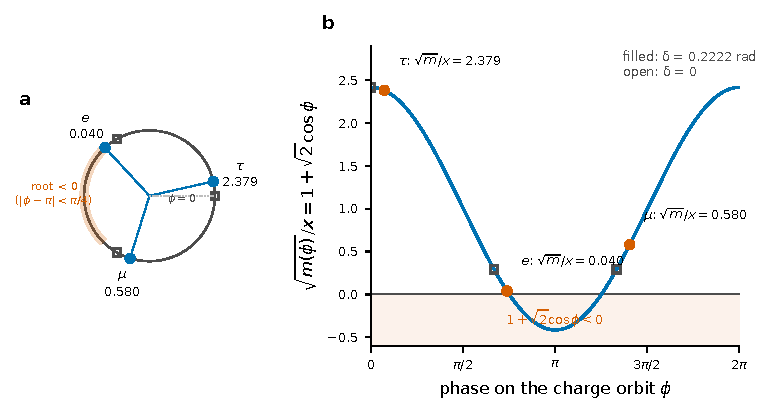
\includegraphics[width=\textwidth]{figures/part2/fig_koide_orbit.pdf}
\caption[The charge orbit and the three phases]{(a) The charge orbit $S^1$ with the three phases $\phi_k=\delta+2\pi k/3$ at the measured offset
$\delta=0.2222$\,rad (filled) and at $\delta=0$ (open squares), with $\sqrt{m_k}/x$ for the $\tau$ ($k=0$), electron ($k=1$) and muon ($k=2$). The
shaded arc, $|\phi-\pi|<\pi/4$, is where $1+\sqrt2\cos\phi<0$. (b) The encoding $\sqrt{m(\phi)}/x=1+\sqrt2\cos\phi$ with the same points: 2.379, 0.040
and 0.580 at the measured offset; at $\delta=0$ the electron and muon coincide at 0.293. PDG 2024 masses~\cite{PDG2024}. \calc}\label{fig:ko:orbit}
\end{figure}

\begin{figure}[htbp]\centering
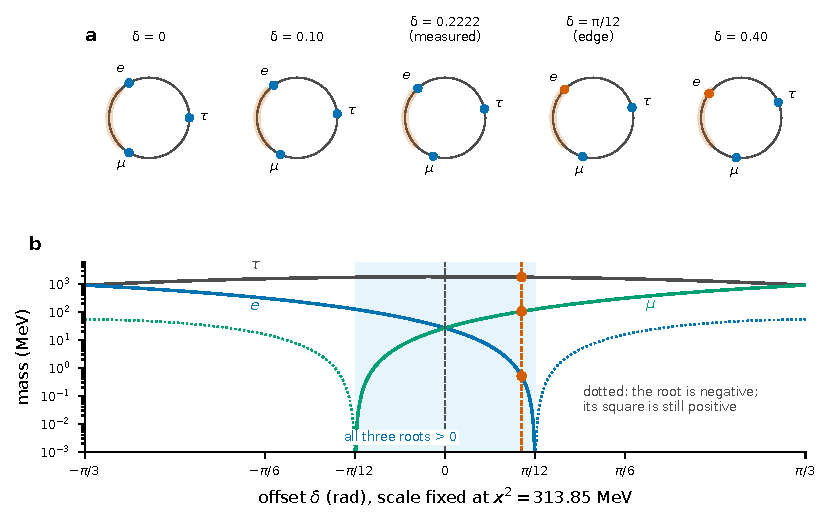
\includegraphics[width=\textwidth]{figures/part2/fig_koide_sweep.pdf}
\caption[The offset sweep]{The offset $\delta$ at fixed scale $x^2=313.85$\,MeV and $y/x=\sqrt2$. (a) The orbit at $\delta=0$, 0.10, 0.2222
(measured), $\pi/12$ (the electron amplitude reaches zero) and 0.40 (the electron amplitude is negative, orange). (b) The three masses against
$\delta$: solid where the amplitude is positive, dotted where it is negative (the mass, its square, stays positive). The shaded window
$|\delta|<\pi/12$ is where all three amplitudes are positive; the dashed lines mark $\delta=0$, where $m_e=m_\mu=26.92$\,MeV, and the measured offset,
where the curves pass through the measured masses (points). The pattern repeats with period $2\pi/3$, which relabels the leptons. Static version of
the animation in the source archive. \calc}\label{fig:ko:sweep}
\end{figure}

\begin{table}[htbp]\centering\small
\caption{The circle parameters and the offset. PDG 2024 masses; \texttt{verify\_particle\_book.py}.}\label{tab:ko:fit}
\begin{tabular}{llll}\toprule
quantity & value & from & label\\\midrule
scale $x$, $x^2$ & $17.71584$\,MeV$^{1/2}$, $313.851$\,MeV & $\sum_k\sqrt{m_k}/3$ & \calc\\
ratio $r=y/x$ & $1.414209$ ($\sqrt2=1.414214$) & Eq.~\eqref{eq:ko:Qr} & \calc\\
offset $\delta$ & $0.222225\pm0.000006$\,rad & first harmonic of the samples & \calc\\
angle to $(1,1,1)$ & $44.99991^\circ$ & Eq.~\eqref{eq:ko:angle} & \calc\\
masses at $\delta=0$ & $26.92$, $26.92$, $1829.26$\,MeV & Eq.~\eqref{eq:ko:delta0} & \calc\\
edge of the positive window & $\delta=\pi/12=0.2618$; measured $\delta$ is $0.0396$ inside & Eq.~\eqref{eq:ko:pos} & \calc\\
offset if $Q=2/3$ exactly & $0.222222047\pm0.0000000004$\,rad (from $m_e$, $m_\mu$) & K13 & \calc\\
$2/9-\delta$ at $Q=2/3$ exactly & $1.75\times10^{-7}$\,rad & K13 & \calc\\\bottomrule
\end{tabular}
\end{table}

\paragraph{The value $2/9$.} If $Q=2/3$ holds exactly, the electron and muon masses alone fix the offset to $\delta=0.222222047$, with an
uncertainty of $4\times10^{-10}$\,rad from $m_\mu$. That is $1.75\times10^{-7}$\,rad below $2/9$. \calc{} $Q=2/3$ and $\delta=2/9$ cannot both hold
exactly. With the three masses fitted freely, $\delta=2/9$ is within $0.4\sigma$; the decisive number is $m_\tau$. \calc

\section{What the boundary reading adds}\label{sec:ko:reading}
On the reading of this chapter, the three charged leptons are three phase states of one encoding on the charge orbit of $|Q|=1$, and $Q=2/3$ is the
statement that the constant channel and the modulating channel carry equal information. \interp{} It connects Koide's relation to the same
principles that set the Bekenstein--Hawking coefficient. It does not predict the absolute scale, which would need a boundary action fixing $x$,
and it does not predict the offset. It applies to a fixed charge $|Q|=1$; whether the same reading extends to the quarks, whose charges are
$2/3$ and $1/3$ and whose masses must be compared at a common scale, is not treated. \openprob

\section{Predictions and tests}\label{sec:ko:tests}
\begin{enumerate}
\item \textbf{The $\tau$ mass.} With $Q=2/3$ exactly, $m_e$ and $m_\mu$ fix $m_\tau=1776.9690$\,MeV. The 2024 average is $1776.93\pm0.09$\,MeV, a
pull of $-0.43\sigma$; the 2022 average, $1776.86\pm0.12$\,MeV, gave $-0.9\sigma$. \calc{} A measurement at $\pm0.01$\,MeV with the present
central value would separate them at $3.9\sigma$; the most precise single measurement today is $1777.09\pm0.08\pm0.11$\,MeV~\cite{BelleII2023tau}.
\prediction{} The test is of $Q=2/3$, not of the route to it: any mechanism that gives $y/x=\sqrt2$ makes the same prediction.
\item \textbf{The offset.} A $\tau$ mass that settles at $1776.969$\,MeV would also settle $\delta=0.2222220$ and exclude $\delta=2/9$ exactly at
the level set by $m_\mu$. \calc
\item \textbf{The model layer.} Four statements would break the route, and they are its tests. (i) A controlled de Sitter construction in which a
charged operator sector does not reduce to an $S^1$ carrying one phase. (ii) A boundary action that populates the second and higher harmonics
above $w_2/w_1\sim10^{-10}$; since three masses cannot see the harmonics directly, this is a test of the action, not of the masses. (iii) A
multi-channel horizon encoding whose entropy, computed from microstates, is not maximised by the equal partition; that would also bear on the
standard account of black-hole entropy. (iv) Independent flavour constructions (discrete or modular family symmetries, holographic models)
that reach $Z_3$ phases with $y/x=\sqrt2$ without imposing them would support the route; constructions that consistently reach other ratios or
counts would weigh against it. \openprob
\end{enumerate}

\section{Status}\label{sec:ko:status}
\begin{center}\small\begin{tabular}{p{0.62\textwidth}l}\toprule
statement & label\\\midrule
$Q=0.66666446\pm0.00000508$ for the pole masses; $2/3$ within $0.43\sigma$ & \observed\\
$Q=2/3\Leftrightarrow$ the square-root vector at $45^\circ$ to $(1,1,1)$ $\Leftrightarrow r=\sqrt2$ & \derived\\
Theorems 1 and 2 (count and value), given $y/x=\sqrt2$ and positive amplitudes & \derived\\
$\eta=1/4\lP^2$ from the Euclidean period and the Einstein normalisation; one nat per $4\lP^2$ & \derived\\
charge-orbit reduction; boundary record and $S\propto A$; maximum-entropy equipartition; two-mode ground state; Parseval identification & \conjecture\\
$y/x=\sqrt2$ from equal channel weights & \derived{} (given the conjectures)\\
the virial reading $2x^2=y^2$ & \analogy\\
the offset $\delta=0.2222$ and the scale $x$; why pole masses; $\delta\approx2/9$ & \openprob\\
$m_\tau=1776.969$\,MeV from $Q=2/3$ & \prediction\\\bottomrule
\end{tabular}\end{center}
The chain closes the value $2/3$ and the bound on the count. It does not close the spectrum: with the offset that its own symmetry selects, the
electron and the muon would weigh the same.
